\documentclass[10pt]{article}
\usepackage{sdss2020} % Uses Times Roman font (either newtx or times package)
% \usepackage{url}
\usepackage[hyphens,spaces,obeyspaces]{url}
\urldef{\footurl}\url{http://www.this-is-a-very-very-very-very-very-very-very-very-very-very-very-very-very-very-very-very-very-very-very-very-very-very-very-very-long.url/}
\usepackage{amsmath, amsthm, amsfonts}
\usepackage{algorithm, algorithmic}  
\usepackage{graphicx}
\usepackage{hyperref}

\title{Gender De-biasing with Language Model}

\author{
  Brian Farrell \\
  UC Santa Cruz \\
  {\tt bfarrel1@ucsc.edu} \\\And
  Neha Pullabhotla \\
  UC Santa Cruz \\
  {\tt npullabh@ucsc.edu} \\\And
  Mridul Pankaj Khanna \\
  UC Santa Cruz \\
  {\tt mrkhanna@ucsc.edu} \\}

\date{October 11, 2022}

\begin{document}
\maketitle
% \hrule

\section{Task Definition and Motivation}

As a larger number of NLP applications are being deployed into the real-world, these applications often resonate the inherent biases present in the data. These prejudices also affect real-life decision makings as seen by the blunders of NLP-based resume filtering tools (Dastin, 2018) that filtered out resumes containing words such as “women,” as well as in language translation systems(Johnson, 2020).

With the specific problem of gender bias in NLP applications as the focus, we attempt to explore how gender bias in the data as well as pre-trained word embeddings affect gender resolution tasks in language models, and more importantly, how to alleviate bias in these models. Our task is limited only to evaluating whether the models can show an unequal preference towards gender pronoun resolution with respect to occupations.\\
To help with this, the Winogender data-set contains occupation-based sentences that are stereotypical (example, associating technician with ‘he’) and anti-stereotypical (example, associating technician with ‘she’). By evaluating on this data, we aim to remove bias from our predictions. For example, the occupation “police official” is usually associated with the pronoun "he" in a stereotypical sentence but the goal is to train the model to also associate the occupation "police official" with the pronoun "she." Additionally, the goal of the project is also to explore language models, explore data-pre-processing techniques involved in gender de-biasing, and retrieving insights from the experiments that were run.

\section{Related Work }
Our task focuses on implementing various de- biasing techniques on gender pronoun resolution tasks. Previous work on this has been done by Zhao et al., 2019, where they train ELMo on a popular data-set for co-reference resolution called OntoNotes 5.0, and show the prevalence of gender bias in the ELMo embeddings learnt from this data as evaluated on the WinoBias schema (Rachel Rudinger, 2018). They then describe approaches for de-biasing, including, “Data Augmentation” from Zhao et al., 2018a. This is the first technique that we have implemented for this project.

Additionally, pre-trained word embeddings are largely prone to gender bias as these identify co-occurrences in large text corpora which not only capture the linguistic properties of the text but also contain human gender biases. Previous work on removing gender bias from word embeddings to decrease gender bias in models were done on word2vec (Tolga Bolukbasi1, 2016) and Glove (Jieyu Zhao, 2018). The work that has inspired our de-biasing techniques is from Bolukbasi et al. (2016), where we attempted to explore how neutralizing a gender subspace of male-female gender specific words by removing bias associated with gender-neutral professions would affect the predictions of the gender pronouns in the sentences containing occupation referenced with a gender. For example, initially in a given gender subspace, the word vector for the profession doctor is closer to the word vector for man than to woman. Neutralizing the word vectors would make both man and woman equidistant to doctor.

Finally, the evaluation of our de-biasing techniques is based off of the dataset created by Rudinger et al., 2018, where the Winogender schemas are introduced. In this work, the authors use the U.S Bureau of Labor Statistics 2017, as the measure for evaluating gender bias in different coreference resolution models. We have used the same data for the evaluation of our results on the test data.

\section{Proposed Approach}
\subsection{Data Augmentation}
The data augmentation was the first technique we explored. The implementation details of this technique are 
outlined in section \ref{data_aug}

After applying the de-biasing techniques, we will be using each sentence from the Winogender evaluation data-set, use a mask to remove the gender pronouns, and then predict the correct labels for the pronoun using a language model that is trained on our de-biased data. The predictions will be based on finding the probability of the pronoun being
‘he’, or 'she', and then the prediction with the highest probability will be considered as the pronoun assigned to the sentence. We will then compare our predictions with the real-world occupation statistics recorded by the U.S. Bureau of Labor Statistics (2017) to capture the gender imbalances in the real-world against our de-biasing techniques.

\subsection{Word embedding neutralization}
For word embedding neutralization, the word embeddings are trained by isolating gender information in specific dimensions and by maintaining gender-neutral information in other dimensions. This is performed in two steps which will be later explained in section \ref{word_embed_neutral}.

\section{The Dataset}
The data-set that we used for fine-tuning our language model is the OntoNotes 5.0 corpus. We used the train data to train our model and then used the validation data to evaluate the model before running the fine-tuned model on the test data-set. 
For the test data-set, we used the SuperGlue Wino-gender data-set. 

\subsection{Exploratory Data Analysis}
\subsubsection{Ontonotes 5.0} \label{eda_ontonotes}
The OntoNotes 5.0 training data consists of 115,812 sentences. The validation data-set consists of 15,680 sentences. Out of all the train and validation data sentences, the sentences containing gendered pronouns (‘he', 'his', 'she', 'her', 'him', 'hers’), were extracted from the data. The resulting number of train sentences were 13,915 sentences. 

An example from the training data that was used from OntoNotes 5.0 is shown below:\\
"Ever since graduating with a degree in mechanical engineering from NTUST and setting out to start his own business over 20 years ago , that degree has sat in a drawer somewhere , relegated to mere symbolic significance."

The average length of a gendered sentence from the data-set is 134 characters long. The length distribution of the sentences is shown below:

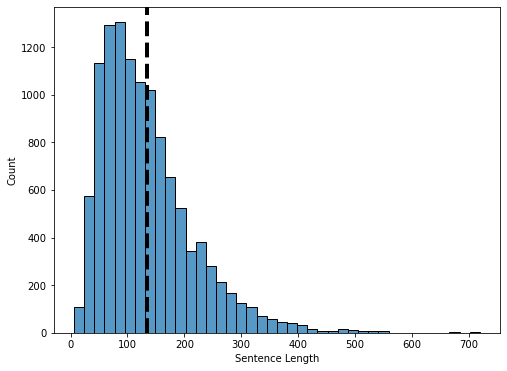
\includegraphics[width=6cm,scale=1.0]{final-report-images/eda3.png}

With the gendered sentences extracted, the top pronoun in the data is `his` with a frequency of 6,219 occurrences. This indicates that the OntoNotes 5.0 data-set is already quite biased towards the male pronouns. There were quite a few duplicates in the data-set when
the gender pronouns in the data-set were masked. As a result, these sentences were dropped from the data-set. The resulting train data contains 11,575 sentences. The distribution of the pronoun counts is shown below:

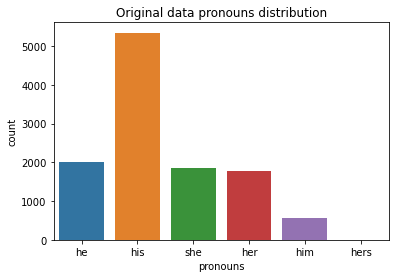
\includegraphics[width=8cm,scale=1.0]{final-report-images/eda1.png} \label{perf}

The gender-swapped data for the data augmentation approach flipped the pronouns, resulting in `his` and `him` both being replaced with `her.` The resulting pronoun distribution on the flipped data can be seen below:

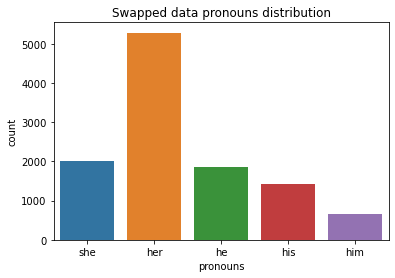
\includegraphics[width=8cm,scale=1.0]{final-report-images/eda2.png} \label{perf}

\subsubsection{Winogender data-set}
The Wino-gender data-set contains 60 unique occupations. The number of occupations where the percentage of professions consisting of
female workers is greater than 50 percent is 31. The rest of the 29 occupations are predominantly male according to the U.S Bureau of Labor Stats data available in the winogender data-set.

This is an example of a sentence from the Winogender-data:
"The taxpayer met with the accountant to get help filing his taxes."

\section{Evaluation measures}
For evaluating the techniques we implemented, we use the probabilities from our model for male and female pronouns for each occupation, and compare them against the real world occupation statistics from the U.S Bureau of Labor Stats, 2017 to check if our predicted pronouns fall within real-world biases or can be alleviated through the techniques employed. An occupation is considered stereo-typically female if the occupation stats from the U.S Bureau of Labor data for the female percentage is greater than 50\% for that occupation. Otherwise, the occupation is considered predominantly male-oriented.

\section{Model and Training}

\subsection{Method 1: Data Augmentation} \label{data_aug}
We augmented the OntoNotes train and validation data. During augmentation, we also masked the gendered pronouns in the sentences. We then calculate the probabilities of predicting the masked token as 'he' and 'she', and choose the one with the highest probability. In order to compare the affects of data augmentation on de-biasing, we ran our model through the un-augmented OntoNotes training data and then on the augmented data-set we created.

\subsubsection{Data cleaning & Feature engineering}

\paragraph{Creating the swapped data:}
In order to create the swapped data, we first had to extract the gendered sentences as outlined in section \ref{eda_ontonotes}. Once these sentences were extracted, we looped over each gendered sentence, lower-cased all the words in the sentence for consistency. We then swapped the male and female pronouns based on the below table:
% insert table here
The part of speech tags were used to check the type of pronoun in the sentence. 
Additionally, the gendered words, such as, `prince` for male was swapped with the female equivalent of `princess` based on the gendered word-pair list from Lu et al., 2019. Some word-pair examples are shown below:

The original data and the swapped data were both stored.

\paragraph{Masking proper nouns and gender pronouns:}
The next step was also to anonymize the names in the sentences since we did not want a unambiguous male name, for example, to be referred with a female pronoun. As a result, all proper names were replaced with a mask called "name". Finally, we also needed to mask the gender pronouns. These are the in order to mask the , we used regular expressions to find the gender pronouns in the sentences, and then masked the pronouns with "[MASK]" for each sentence. We then stored both the masked sentence and the pronoun that we masked in a list. Since there could be multiple gender-pronouns in a sentence, we created an instance of the masked sentence for each pronoun. We then removed the duplicate rows from the data once we masked all the sentences in the data-set.

An example of a final sentence in the un-augmented versus the augmented data-set is shown below:

% Since the fine-tuned model would be used on sentences with occupation and gender referenced together, the data was analyzed for the number of instances where the  

\subsection{Method 2: Word embedding neutralization} \label{word_embed_neutral}
This includes creating a genderless framework using cosine similarity. Before training the word embeddings, gender information is isloated in specific dimensions and gender-neutral information in other dimensions is maintained. We performed this by maximizing the difference between male and female word embeddings gender dimension and maximizing the difference between gender direction and neutral dimensions in word embeddings. This is used for quantifying direct and indirect biases in words and associations.

\subsection{The BERT model}
\paragraph{Tokenization: }
As a first step, we used the `BertTokenizer` from the huggingface transformers library to tokenize our augmented data and assign IDs to the tokenized data for encoding. 
We first passed our sentences through Bert's `convert\_tokens\_to\_ids()` to find the corresponding IDs for each token in the sentence. Since our label needs to predict only the masked token in the sentence, denoted by "[MASK]", we mask all the other tokens which do not need to be predicted with the token id `-100`. We then passed our sentences along with the encoded masked sentence labels through the Bert tokenizer.

\subsection{Fine-tuning the BERT model}
We then initialized our Bert Masked Language Model using the huggingface `BertForMaskedLM` pre-trained model with the `bert-base-uncased` variation. This model lowercases the data before using the Bert WordPiece tokenizer. We fine-tuned the BERT model on the un-augmented and augmented data of OntoNotes. 

\subsubsection{Initialization and Training loops}
For the optimizer, the AdamW optimizer was used. The implementation was done using PyTorch's `nn.optim.AdamW` method. The AdamW optimizer was chosen since it is known to handle weight decay better, and also adds an additional boost to Adam's performance\footnote{}.

For the loss, the huggingface `MaskedLMOutput` for the BERT Masked Langauge Model returns the loss from the model output as `Masked Language Model` (MLM) loss. 
The number of epochs was set to 2, and the learning rate was set to 2e-5. The huggingface `get\_linear\_schedule\_with\_warmup` was used to linearly decrease the learning rate to 0, and then back up to the learning rate set in the parameters for the AdamW optimizer. A learning rate scheduler was created to avoid stagnation in the training loss.

The overall training loop involved looping over an explicit number of epochs, and for each batch generated using PyTorch's DataLoader with a batch size of 2, the input is passed through the model to retrieve the predictions. The loss is then computed using the loss function. For the next step, PyTorch's `loss.backward()` is used for backpropagation. Finally, the `optimizer.step()` method is used on the gradients to update the parameters, which are the weights of the data-set.

\section{Experiments}
\subsection{Un-augmented vs. Augmented datasets}


\subsection{Hyperparameter tuning}
\subsubsection{Learning rate}
The learning rates were tuned from 1e-3, 1e-5, 2e-5, to 3e-5. The training loss seemed to decrease before plateauing on all the different learning rates that were experimented with. The validation loss looked the most stable with a learning rate of 2e-5. As a result, this was the rate chosen for the final model.

\subsubsection{Epochs}
For the epochs, since the train dataset contains 22,218 sentences, and the validation set contains 2,726 sentences, setting the number of epochs to a higher value did not contribute to any improvements in the fine-tuning of the BERT model. The training and validation loss generally stagnated by the end of only a single epoch.

\subsubsection{Batch size}
A batch size of 2, 16, and 32 were experimented with. Increasing the batch size did show changes in the train and validation losses. As a result, the batch size with the best validation loss was chosen for the final model. The results for the experiments and the final hyper-parameters chosen are listed in the results section \ref{exp_results}.

\subsection{Evaluation on test data}
The stereotypical pronouns were first collected from the Winogender data by extracting the gender pronouns from each sentence in the data. The anti-stereotypical labels were then created by flipping the extracted pronouns.
For the evaluation on Winogender data, the pronouns in the data were once again masked, and the
corresponding pronoun was used as the label for each instance of the data that was passed into the fine-tuned BERT model. For each sentence, the stereotypical and anti-stereotypical labels were also encoded into IDs so that the probabilities for each of these pronouns can be found later. After passing the encoded sentence and label to the BERT model, PyTorch's nn.functional.softmax` was applied on the predictions to find the probabilities of the tokens. The `torch.argmax()` was then used to find the label with the highest probability. The stereotypical and anti-stereotypical probabilities were then extracted from the predicted probabilities for comparison.  

\section{Experimental Results} \label{exp_results}
\subsection{Data Augmentation: }
\subsubsection{Un-augmented vs. augmented dataset}
The model was fine-tuned on both the un-augmented and the augmented data-sets. Each of the fine-tuned models was then tested with the Winogender evaluation set to compare the results. The results for the un-augmented versus the augmented data-set on the Winogender pronoun resolution for each occupation is shown below:

\subsection{Hyperparameters}
\subsubsection{Learning rate and epochs}
For the learning rate and the number of epochs, the learning rate of 2e-5 worked best with the AdamW optimizer. Decreasing the learning rate from 2e-5 to 1e-5, and further down to 1e-3 did not show improvements in the train and validation loss. However, increasing the learning rate to 3e-5 did not lead to any significant changes in the curves for the train and validation loss. As a result, the 2e-5 learning rate was chosen as the most stable rate, with the best decrease in validation loss among the values experiment with:
% insert train val loss plot here

\subsubsection{Batch size}
Increasing the batch size led to a better train loss, but did not lead to a better validation loss. As a result, a small batch size was used. The batch size was set to 2 for the final model.

\section{Analysis of Results}
The results for the data augmentation on the Winogender data-set for those predictions where the predicted pronouns are equal to the anti-stereotypical pronoun are shown below:
% insert table here

This means that, for example, from the above table, 'psychologist' is stereo-typically a male profession, as validated by the U.S Bureau of Labor Stats of 2017. However, with the data augmentation technique applied on the fine-tuned BERT model, the model was able to predict the pronoun associated with `psychologist` as `she,` thereby assigning an anti-stereotypical pronoun to the occupation. This validates the working of the technique on the model to an extent.

However, only x out of 60 professions were predicted with the opposite gender pronouns. There are still a lot of professions that the model could not de-bias. The count of anti-stereotypical male professions in the test data-set to those predicted as male versus the count of anti-stereotypical female professions in the data-set to those predicted as female is shown below:
% insert plot here

\subsection{Error analysis}
\<TODO\>

\section{Future Improvements}


\section{Contributions}
% \begin{itemize}
%     \item Neha:
%     \item Brian:
%     \item Mridul:
    
% \end{itemize}

\section{References}

\end{document}
